\documentclass[conference]{IEEEtran}
% DIC4 draft -- Hybrid TPA-Agent. Source of truth for the system design:
% openspec/changes/add-hybrid-tpa-agent-core/ ; paper rules: openspec/changes/add-ieee-conference-draft/
\IEEEoverridecommandlockouts
\usepackage{cite}
\usepackage{amsmath,amssymb,amsfonts}
\usepackage{algorithm}
\usepackage{algpseudocode}
\usepackage{graphicx}
\usepackage{textcomp}
\usepackage{xcolor}
\usepackage{booktabs}
\usepackage{url}
\usepackage{tikz}
\usetikzlibrary{positioning,arrows.meta,fit,backgrounds}

\begin{document}

\title{Hybrid TPA-Agent: Decoupling Deterministic Structure, Machine-Learned Probability, and LLM Reasoning for Risk-First Short-Term Trading Decision Support}

\author{\IEEEauthorblockN{Chia-Min Hou}
\IEEEauthorblockA{\textit{Department of Computer Science and Engineering} \\
\textit{National Chung Hsing University}\\
Taichung, Taiwan}
% Team members of the course project can be added here as additional \IEEEauthorblockN blocks.
}

\maketitle

\begin{abstract}
Day trading has become a dominant activity in the Taiwan stock market, accounting for 32.77\% of turnover in 2025, yet decades of evidence show that fewer than 1\% of retail day traders remain profitable after costs. Non-professional traders must locate price structure, judge the probability of a reaction, and size risk within seconds, a combination that existing tools address only in part: technical-indicator models ignore where price sits in the market structure, support--resistance algorithms output static lines without probabilities, and large language model (LLM) trading agents produce unreliable numbers and backtests inflated by memorized market history. This paper proposes the Hybrid Technical \& Price Action Agent (Hybrid TPA-Agent), a decision-support system built on the principle that each component does only what it does best. Deterministic algorithms detect supply and demand zones, an XGBoost classifier estimates the probability of a rebound or breakout, an LLM reasons over structured data and a price-action knowledge base without producing any price or probability, and a deterministic risk engine derives stop-loss, take-profit, risk--reward ratio, and position size. A setup is approved only when the win probability is at least 0.55 and the risk--reward ratio is at least 2.0, and every approval requires human confirmation. We specify the system as eight testable capabilities and present an evaluation plan with time-ordered splits, transaction costs, component ablations, and test periods after the LLM's knowledge cutoff. Experimental results will be reported after implementation.
\end{abstract}

\begin{IEEEkeywords}
LLM agents, algorithmic trading, price action, supply and demand zones, XGBoost, decision support, human-in-the-loop, look-ahead bias
\end{IEEEkeywords}

\section{Introduction}

Short-term day trading is now a mainstream activity in Taiwan. According to Taiwan Stock Exchange statistics, day trading accounted for 32.77\% of total turnover in 2025, with about 150{,}000 accounts trading intraday on an average day~\cite{yahoo2025daytrade}, and its share of a single day's listed-market turnover reached 45.22\% in November 2026~\cite{ctee2026daytrade}. Participation, however, does not imply profitability. Using complete transaction records of the Taiwan Stock Exchange from 1992 to 2006, Barber \emph{et al.} found that only about 13\% of day traders earned profits net of fees in a typical year and that fewer than 1\% outperformed persistently~\cite{barber2014speculator}. Among Brazilian futures day traders who persisted for more than 300 days, 97\% lost money~\cite{chague2019daytrading}.

A short-term decision requires three judgments within seconds to minutes: a \emph{structural} judgment about where support, resistance, supply, and demand lie; a \emph{probabilistic} judgment about whether price will rebound or break through at that location; and a \emph{risk} judgment that fixes the invalidation point, the risk--reward ratio, and the position size before entry. Each demands different expertise, and under time pressure and emotional stress, non-professional traders rarely perform all three consistently.

Prior work addresses these judgments separately. Machine learning (ML) classifiers predict price direction from technical indicators~\cite{soltanisehat2025multimodel}; support--resistance (S/R) algorithms locate horizontal levels~\cite{chan2022support,kriuk2025deepsupp}; and LLM agents emulate trading teams~\cite{xiao2024tradingagents} or read chart images~\cite{chen2025mmdrex}. Each leaves a gap. Indicator-based models do not know where price sits in the market structure; S/R detectors output lines rather than zones and do not estimate the probability of a successful retest; and LLMs are unreliable at arithmetic and probability calibration~\cite{kuang2025hybrid}, while their backtests can be inflated because the models memorize historical market outcomes~\cite{lopezlira2025memorization,gao2025lookahead,li2025profitmirage}. Under broader and longer evaluation, previously reported LLM advantages deteriorate markedly~\cite{li2025finsaber}, and a recent survey notes that most agentic systems focus on signal generation and rarely cover risk management~\cite{hua2026agentic}.

We propose the Hybrid TPA-Agent, which assigns each judgment to the component best suited to it and keeps the LLM away from numbers. Our contributions are:
\begin{itemize}
\item A four-layer, eight-module agent architecture that separates deterministic spatial structure, machine-learned probability, and constrained LLM reasoning, reducing exposure to numerical hallucination and memorization-driven backtest bias.
\item A codification of price-action knowledge---supply and demand zones, support--resistance role flips, and false breakouts---into reproducible rules and structured features for win-rate estimation.
\item A risk-first decision procedure based on expected value, dual thresholds, and risk-budget position sizing, with human confirmation and graded degradation under data faults.
\item An open, spec-driven design: every module is specified as a testable OpenSpec capability with scenarios, so that later developers can implement and verify the system.
\end{itemize}

The remainder of this paper is organized as follows. Section~\ref{sec:related} reviews related work. Section~\ref{sec:principles} states the design principles. Section~\ref{sec:system} presents the architecture and core algorithm. Section~\ref{sec:eval} describes the evaluation plan, and Section~\ref{sec:conclusion} concludes.

\begin{figure*}[t]
\centering
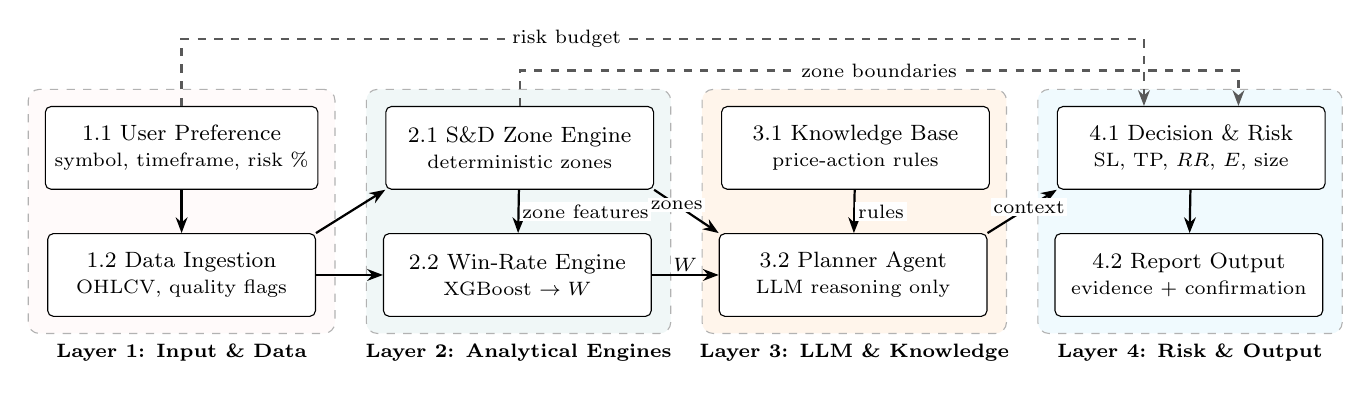
\begin{tikzpicture}[
  font=\footnotesize,
  mod/.style={draw, rounded corners=2pt, align=center, minimum width=3.4cm, minimum height=1.05cm, fill=white},
  lay/.style={draw=gray!60, dashed, rounded corners=4pt, inner sep=6pt},
  arr/.style={-{Stealth[length=2mm]}, thick},
  lbl/.style={font=\scriptsize, fill=white, inner sep=1pt},
  node distance=0.55cm and 0.85cm]
\node[mod] (m11) {1.1 User Preference\\\scriptsize symbol, timeframe, risk \%};
\node[mod, below=of m11] (m12) {1.2 Data Ingestion\\\scriptsize OHLCV, quality flags};
\node[mod, right=of m11] (m21) {2.1 S\&D Zone Engine\\\scriptsize deterministic zones};
\node[mod, right=of m12] (m22) {2.2 Win-Rate Engine\\\scriptsize XGBoost $\rightarrow W$};
\node[mod, right=of m21] (m31) {3.1 Knowledge Base\\\scriptsize price-action rules};
\node[mod, right=of m22] (m32) {3.2 Planner Agent\\\scriptsize LLM reasoning only};
\node[mod, right=of m31] (m41) {4.1 Decision \& Risk\\\scriptsize SL, TP, $RR$, $E$, size};
\node[mod, right=of m32] (m42) {4.2 Report Output\\\scriptsize evidence + confirmation};
\begin{scope}[on background layer]
\node[lay, fill=pink!8, fit=(m11)(m12), label={[font=\scriptsize\bfseries]below:Layer 1: Input \& Data}] {};
\node[lay, fill=teal!6, fit=(m21)(m22), label={[font=\scriptsize\bfseries]below:Layer 2: Analytical Engines}] {};
\node[lay, fill=orange!8, fit=(m31)(m32), label={[font=\scriptsize\bfseries]below:Layer 3: LLM \& Knowledge}] {};
\node[lay, fill=cyan!6, fit=(m41)(m42), label={[font=\scriptsize\bfseries]below:Layer 4: Risk \& Output}] {};
\end{scope}
\draw[arr] (m11) -- (m12);
\draw[arr] (m12) -- (m22);
\draw[arr] (m12.north east) -- (m21.south west);
\draw[arr] (m21) -- node[lbl, right] {zone features} (m22);
\draw[arr] (m21.south east) -- node[lbl, pos=0.35] {zones} (m32.north west);
\draw[arr] (m22) -- node[lbl, above] {$W$} (m32);
\draw[arr] (m31) -- node[lbl, right] {rules} (m32);
\draw[arr] (m32.north east) -- node[lbl, pos=0.6] {context} (m41.south west);
\draw[arr] (m41) -- (m42);
\draw[arr, dashed, gray!70!black] (m21.north) -- ++(0,0.45) -| node[lbl, pos=0.25, text=black] {zone boundaries} ([xshift=6mm]m41.north);
\draw[arr, dashed, gray!70!black] (m11.north) -- ++(0,0.85) -| node[lbl, pos=0.2, text=black] {risk budget} ([xshift=-6mm]m41.north);
\end{tikzpicture}
\caption{Four-layer, eight-module architecture of the Hybrid TPA-Agent. Solid arrows show the main data flow. Dashed arrows show zone boundaries and the user's risk budget passed directly to the deterministic risk engine, so that no price or position size depends on LLM output.}
\label{fig:arch}
\end{figure*}

\section{Related Work}\label{sec:related}

\subsection{Evidence on Short-Term Traders}
Large-scale studies consistently find that few retail day traders profit after costs~\cite{barber2014speculator,chague2019daytrading}. The problem is therefore less a lack of information than a lack of disciplined, verifiable decision processes, which motivates our risk-first design.

\subsection{Market Mechanisms Behind Support and Resistance}
Osler showed with actual currency order data that take-profit and stop-loss orders cluster near round numbers, which explains why prices tend to reverse at, or accelerate through, such levels~\cite{osler2003currency}. Supply and demand zones are thus locations where unfilled orders accumulate, not merely lines on a chart. For labeling, the triple-barrier method defines a trade's outcome by whichever of a take-profit, stop-loss, or time barrier is reached first, and meta-labeling lets a model decide whether to act on a candidate signal~\cite{lopezdeprado2018advances}. Our win-rate model follows this division: zones propose candidates, and the classifier estimates their success probability.

\subsection{Machine Learning for Structure and Direction}
Chan \emph{et al.} detected S/R levels with a swing-high/swing-low algorithm and fed distances to the nearest levels into a GRU encoder--decoder, improving take-profit precision on four currency pairs; however, higher precision did not always yield higher profit because risk--reward ratios differed across trades~\cite{chan2022support}. DeepSupp extracts support levels with multi-head attention over dynamic correlation matrices followed by DBSCAN clustering~\cite{kriuk2025deepsupp}. Soltanisehat and Rai compared nine classifiers on 36 technical indicators and found XGBoost best for two of three stocks~\cite{soltanisehat2025multimodel}. These works show that structural information helps prediction, but they output lines and do not integrate risk-based decisions.

\subsection{LLM Trading Agents}
TradingAgents organizes LLM analysts, bull and bear researchers, and a risk team into a trading-firm workflow~\cite{xiao2024tradingagents}; its backtest covers about three months because each prediction requires many LLM and tool calls. MM-DREX routes strategy experts using a vision--language model over chart images~\cite{chen2025mmdrex}. Hybrid designs are emerging: Kuang and Lin let an LLM construct Bayesian-network structures while all probabilities are computed deterministically~\cite{kuang2025hybrid}, and Jia \emph{et al.} combine LLM-generated reports with rule-based portfolio construction and execution~\cite{jia2026inside}. None of these models price structure explicitly.

\subsection{Reliability of LLM Backtests}
GPT-4o can recall pre-cutoff S\&P~500 index levels with a mean absolute percentage error of about 0.61\%, which rises to about 16.9\% after its knowledge cutoff, and masking or instructed cutoffs do not remove this effect~\cite{lopezlira2025memorization}. A lookahead-propensity test attributes part of LLM news-based return predictability to memorization~\cite{gao2025lookahead}, and LLM agents' backtest returns drop after the model cutoff~\cite{li2025profitmirage}. These findings motivate our choice to keep the LLM away from price and probability estimation.

Table~\ref{tab:compare} summarizes the gap: no existing approach combines deterministic structure, probability estimation, and constrained contextual reasoning under a risk-first decision rule.

\begin{table}[t]
\caption{Capability Comparison with Existing Approaches}
\label{tab:compare}
\centering
\footnotesize
\setlength{\tabcolsep}{3pt}
\begin{tabular}{@{}lccc@{}}
\toprule
Approach & Structure & Probability & Reasoning \& risk \\
\midrule
Indicator ML~\cite{soltanisehat2025multimodel} & -- & \checkmark & -- \\
S/R detection~\cite{chan2022support,kriuk2025deepsupp} & lines & partial & -- \\
LLM agents~\cite{xiao2024tradingagents,chen2025mmdrex} & -- & unreliable & \checkmark \\
LLM + deterministic~\cite{kuang2025hybrid,jia2026inside} & -- & \checkmark & \checkmark \\
\textbf{Hybrid TPA-Agent} & \textbf{zones} & \checkmark & \checkmark \\
\bottomrule
\end{tabular}
\end{table}

\section{Design Principles}\label{sec:principles}

The system follows five core principles, each mapped to modules in Section~\ref{sec:system}.

\textbf{C1 Deterministic spatial structure.} Supply and demand zones are computed by reproducible algorithms; identical inputs and parameters yield identical zones.

\textbf{C2 Machine-learned probability.} A classifier trained on time-ordered data estimates the win probability $W \in [0,1]$ of a candidate setup and is evaluated for calibration as well as accuracy.

\textbf{C3 Decoupled LLM reasoning.} The LLM receives structured JSON and returns a context assessment, reasoning, and cited rule identifiers. It never produces prices or probabilities, and outputs inconsistent with the inputs are rejected.

\textbf{C4 Risk-first decision.} Let $P_e$, $P_{sl}$, and $P_{tp}$ denote the entry, stop-loss, and take-profit prices of a long setup. The risk--reward ratio and expected value per unit of risk are
\begin{equation}
RR = \frac{P_{tp}-P_e}{P_e-P_{sl}}, \qquad E = W \cdot RR - (1-W).
\label{eq:ev}
\end{equation}
A setup is approved only if $W \ge 0.55$ and $RR \ge 2.0$, which implies $E \ge 0.65$.

\textbf{C5 Human-in-the-loop and safe degradation.} The system never submits orders; approved setups are recommendations that require trader confirmation, and new signals are frozen when market data are delayed or interrupted.

These principles resolve three design trade-offs. Signal frequency is sacrificed for expected value (T1); determinism is preferred over flexibility for all numerical quantities (T2); and autonomy is sacrificed for human control and safety (T3).

\section{Proposed System}\label{sec:system}

\subsection{Architecture}
Fig.~\ref{fig:arch} shows the four-layer, eight-module architecture. Each module corresponds to one OpenSpec capability with testable scenarios.


\textbf{Layer 1: Input and data.} The user-preference module (1.1) records the symbol, timeframe, account equity, and maximum risk per trade; no setup can be approved without a risk setting. The ingestion module (1.2) fetches time-ordered OHLCV bars, flags missing, duplicated, or invalid bars, and ensures that every decision at time $t$ uses only bars closed by $t$.

\textbf{Layer 2: Analytical engines.} The zone engine (2.1) detects swing highs and lows with a configurable look-back, confirms candidate zones by volume, and outputs each zone with upper and lower bounds, type, formation time, and test count. A close beyond a zone flips its role between support and resistance. The win-rate engine (2.2) extracts features computed only from past data---distance to the nearest zone, zone width, average true range (ATR), volume z-score, and momentum---and outputs $W$. Training labels follow a barrier rule: a sample wins if the take-profit is reached before the stop-loss within $N$ bars~\cite{lopezdeprado2018advances}.

\textbf{Layer 3: Reasoning and knowledge.} The knowledge base (3.1) stores identified rules such as S/R flips, false breakouts, pin-bar confirmation at retests, and risk-first principles. The planner agent (3.2) receives a structured context containing the current price, zones, $W$, and relevant rules, and returns a context label (e.g., confirmed retest or suspected false breakout), step-by-step reasoning, and cited rule identifiers. Any output whose quoted values differ from the input, and any LLM failure or timeout, results in WAIT/NO\_TRADE.

\textbf{Layer 4: Risk and output.} The decision engine (4.1) places the stop-loss beyond the zone boundary plus an ATR buffer, sets the take-profit at the next opposing zone, computes $RR$ and $E$ by (\ref{eq:ev}), and sizes the position as the risk budget divided by the per-unit stop distance. The report module (4.2) presents the status, prices, $W$, $RR$, $E$, cited zones and rules, and data-quality state, and waits for the trader's confirmation.

\subsection{Core Algorithm}
Algorithm~\ref{alg:tpa} summarizes one analysis cycle.

\begin{algorithm}[t]
\caption{Hybrid TPA-Agent Analysis Cycle}
\label{alg:tpa}
\small
\begin{algorithmic}[1]
\Require symbol $S$, timeframe $TF$, user profile $U$ (equity, risk \%)
\Ensure report $R$ with status APPROVED or WAIT/NO\_TRADE
\State $D \gets$ \textsc{FetchOHLCV}$(S, TF)$; $q \gets$ \textsc{QualityCheck}$(D)$
\If{$q$ is degraded \textbf{or} $U$ lacks a risk setting}
  \State \Return \textsc{Report}(WAIT, reason $=q$ or missing risk)
\EndIf
\State $Z \gets$ \textsc{DetectZones}$(D)$ \Comment{deterministic (C1)}
\State $z \gets$ nearest zone to the last close $p$ in $Z$
\State $x \gets$ \textsc{ExtractFeatures}$(D, z)$; $W \gets$ \textsc{XGBoost}$(x)$ \Comment{C2}
\State $K \gets$ \textsc{RetrieveRules}$(p, z)$
\State $c \gets$ \textsc{LLMReason}$(\{p, Z, W, K\})$ \Comment{no numbers (C3)}
\If{$c$ is invalid \textbf{or} inconsistent with inputs}
  \State \Return \textsc{Report}(WAIT, reason $=$ reasoning failure)
\EndIf
\State $P_{sl} \gets$ zone boundary $\mp$ $k \cdot$ ATR; $P_{tp} \gets$ next opposing zone
\State compute $RR$ and $E$ by (\ref{eq:ev}) \Comment{C4}
\If{$W \ge 0.55$ \textbf{and} $RR \ge 2.0$}
  \State $n \gets \lfloor U.\text{risk} / |p - P_{sl}| \rfloor$
  \State \Return \textsc{Report}(APPROVED, $p, P_{sl}, P_{tp}, n, W, RR, E, c$) \Comment{await confirmation (C5)}
\Else
  \State \Return \textsc{Report}(WAIT, reason $=$ threshold not met)
\EndIf
\end{algorithmic}
\end{algorithm}

\subsection{Specification-Driven Development}
The design is maintained with OpenSpec. Each module is a capability whose requirements are written with SHALL/MUST statements and WHEN/THEN scenarios, for example ``WHEN $W=0.55$ and $RR=2.0$, THEN $E=0.65$'' and ``WHEN the LLM times out, THEN the report status is WAIT/NO\_TRADE.'' The eight capabilities and 27 implementation tasks serve as the acceptance tests for the implementation, and changes to the design are proposed, validated, and archived as versioned change sets.

\section{Experimental Plan}\label{sec:eval}

The evaluation is designed to test whether the hybrid architecture improves decision quality and to avoid the biases identified in Section~\ref{sec:related}. Table~\ref{tab:eval} summarizes the plan.

\begin{table}[t]
\caption{Evaluation Plan}
\label{tab:eval}
\centering
\footnotesize
\setlength{\tabcolsep}{3pt}
\begin{tabular}{@{}p{0.27\columnwidth}p{0.66\columnwidth}@{}}
\toprule
Item & Setting \\
\midrule
Data & Historical OHLCV bars of liquid instruments; market, timeframe, and period to be fixed before experiments \\
Split & Time-ordered training and walk-forward testing; test period after the LLM's knowledge cutoff \\
Baselines & Moving-average crossover; RSI threshold strategy \\
Ablations & Without LLM; without ML (zones only); without zones (indicators only) \\
Metrics & Win-rate accuracy and Brier score; average $RR$; expected value; maximum drawdown; number of signals \\
Costs & Commission, transaction tax, and slippage included \\
Sensitivity & Thresholds $W \in [0.50, 0.65]$, $RR \in [1.5, 3.0]$ \\
\bottomrule
\end{tabular}
\end{table}

\textbf{Bias controls.} All features use only closed bars available at decision time, and the LLM never receives future data or produces numerical forecasts. Selecting test periods after the LLM's knowledge cutoff limits the memorization effects documented in~\cite{lopezlira2025memorization,gao2025lookahead,li2025profitmirage}.

\textbf{Ablations and sensitivity.} Removing each component isolates its contribution, addressing whether the added complexity is justified~\cite{li2025finsaber}. Varying the thresholds quantifies trade-off T1 between the number of signals and expected value.

\textbf{Expected outcomes.} We expect the hybrid system to filter low-quality signals and to provide, for every recommendation, both mathematical evidence ($W$, $RR$, $E$) and price-action reasoning. These are hypotheses; no experimental results are reported in this draft.

\section{Conclusion}\label{sec:conclusion}

This paper presented the Hybrid TPA-Agent, a decision-support system for short-term trading that assigns structural detection to deterministic algorithms, probability estimation to a time-split classifier, contextual reasoning to a constrained LLM, and the final decision to a deterministic, risk-first engine with human confirmation. By keeping the LLM away from prices and probabilities, the design targets two weaknesses of current LLM trading agents: numerical unreliability and memorization-driven backtest inflation. Future work includes implementing the eight specified capabilities, executing the evaluation plan, and extending the data layer with news and order-book information.

\bibliographystyle{IEEEtran}
\bibliography{references}

\end{document}
